% Created 2022-04-06 Wed 18:06
% Intended LaTeX compiler: xelatex
\documentclass[11pt]{article}
\usepackage{graphicx}
\usepackage{longtable}
\usepackage{wrapfig}
\usepackage{rotating}
\usepackage[normalem]{ulem}
\usepackage{amsmath}
\usepackage{amssymb}
\usepackage{capt-of}
\usepackage{hyperref}
\usepackage[newfloat]{minted}
\usepackage{color}
\usepackage{listings}
\usepackage[utf8]{inputenc}
\usepackage[table,xcdraw]{xcolor}
\usepackage{paralist}
\usepackage{datetime2}
\usepackage{graphicx}
\usepackage{lscape}
\usepackage{longtable}
\usepackage{hyperref}
\usepackage[a4paper, left=3cm, right=3cm, top=2cm]{geometry}
\usepackage{fancyhdr}
\usepackage{listings}
\usepackage{textcomp}
\usepackage{enumitem}
\usepackage{algorithm}
\usepackage{algpseudocode}
\setlist{noitemsep}
\setlength{\columnseprule}{0.2pt}
\definecolor{mygreen}{rgb}{0,0.6,0}
\definecolor{mygray}{rgb}{0.5,0.5,0.5}
\definecolor{mymauve}{rgb}{0.58,0,0.82}
\lstset{ backgroundcolor=\color{white}, basicstyle=\footnotesize, breaklines=true, captionpos=b, commentstyle=\color{mygreen}, escapeinside={\%*}{*)},keywordstyle=\color{blue}, stringstyle=\color{mymauve},}
\author{Olivier Lischer}
\date{\today}
\title{Design Patterns - Summary}
\hypersetup{
 pdfauthor={Olivier Lischer},
 pdftitle={Design Patterns - Summary},
 pdfkeywords={},
 pdfsubject={},
 pdfcreator={Emacs 27.2 (Org mode 9.5.2)}, 
 pdflang={English}}
\begin{document}

\pagestyle{fancy}
\fancyhf{}
\fancyhead[R]{SEP2-FS}
\fancyhead[L]{Design Patterns - Summary}
\fancyfoot[CE,CO]{\leftmark}
\fancyfoot[R]{\thepage}
\fancyfoot[L]{Olivier Lischer}

\begin{titlepage}
  \begin{center}
    {\Huge Design Patterns - Summary} \\
    \vspace{8 cm}

    
\includegraphics[height=4cm]{./img/ost-logo.png}

    \vspace{4 cm}
    Semester: Spring 2022
    \vspace{1 cm}

    Version: 0.1.0 \\
    Date: \DTMnow \\
    \vspace{3 cm}
    School of Computer Science\\
    OST Eastern Switzerland University of Applied Sciences
  \end{center}
\end{titlepage}
\newpage
\tableofcontents
\newpage


\section{Introduction}
\label{sec:org0466c2a}
\subsection{Most important quotes}
\label{sec:org8a0def4}
In the introduction the basics of object-oriented programming are explained.
Therefore, for many this is easy to read.
However, some important statements are made.

\begin{quote}
Favor object composition over class inheritance
\end{quote}

Because it is very difficult to make the correct abstraction often the base class(es) are not complete or have too much in it.
With object composition you don't have this problem.

\begin{quote}
Program to an interface, not an implementation
\end{quote}
If you implement against interfaces you can test your class with unit tests.
If you implement against a fixed implementation you can not change this behavior at anytime.


\subsection{The design patterns}
\label{sec:org252e34c}

Class Design Patterns deal with the relationships between classes and their subclasses.
The Object Design Patterns with the object relationships which can be changed at runtime.

\begin{figure}[htbp]
\centering
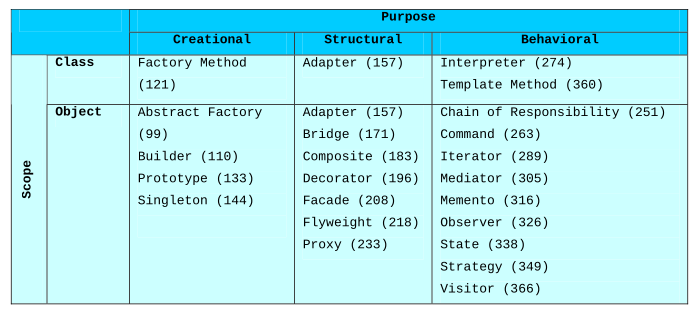
\includegraphics[width=.9\linewidth]{img/design_pattern_space.png}
\caption{\label{fig:org4259c3a}Design pattern space}
\end{figure}
\end{document}